\renewcommand*{\arraystretch}{1.1}

\subsection*{Interactive / complex / 5}
\label{section:interactive-complex-read-05}

% change \emph{} to use sans-serif font
\let\oldemph\emph
\renewcommand{\emph}[1]{{\footnotesize \sf #1}}

\renewcommand{\currentQueryCard}{5}
\marginpar{
	\raggedleft
	\vspace{0.22ex}

	\queryRefCard{interactive-complex-read-01}{Interactive}{1}\\
	\queryRefCard{interactive-complex-read-02}{Interactive}{2}\\
	\queryRefCard{interactive-complex-read-03}{Interactive}{3}\\
	\queryRefCard{interactive-complex-read-04}{Interactive}{4}\\
	\queryRefCard{interactive-complex-read-05}{Interactive}{5}\\
	\queryRefCard{interactive-complex-read-06}{Interactive}{6}\\
	\queryRefCard{interactive-complex-read-07}{Interactive}{7}\\
	\queryRefCard{interactive-complex-read-08}{Interactive}{8}\\
	\queryRefCard{interactive-complex-read-09}{Interactive}{9}\\
	\queryRefCard{interactive-complex-read-10}{Interactive}{10}\\
	\queryRefCard{interactive-complex-read-11}{Interactive}{11}\\
	\queryRefCard{interactive-complex-read-12}{Interactive}{12}\\
	\queryRefCard{interactive-complex-read-13}{Interactive}{13}\\
	\queryRefCard{interactive-complex-read-14}{Interactive}{14}\\
}

\noindent\begin{tabularx}{\queryCardWidth}{|>{\queryPropertyCell}p{\queryPropertyCellWidth}|X|}
	\hline
	query & Interactive / complex / 5 \\ \hline
%
	title & New groups
 \\ \hline
%
	pattern & \hfill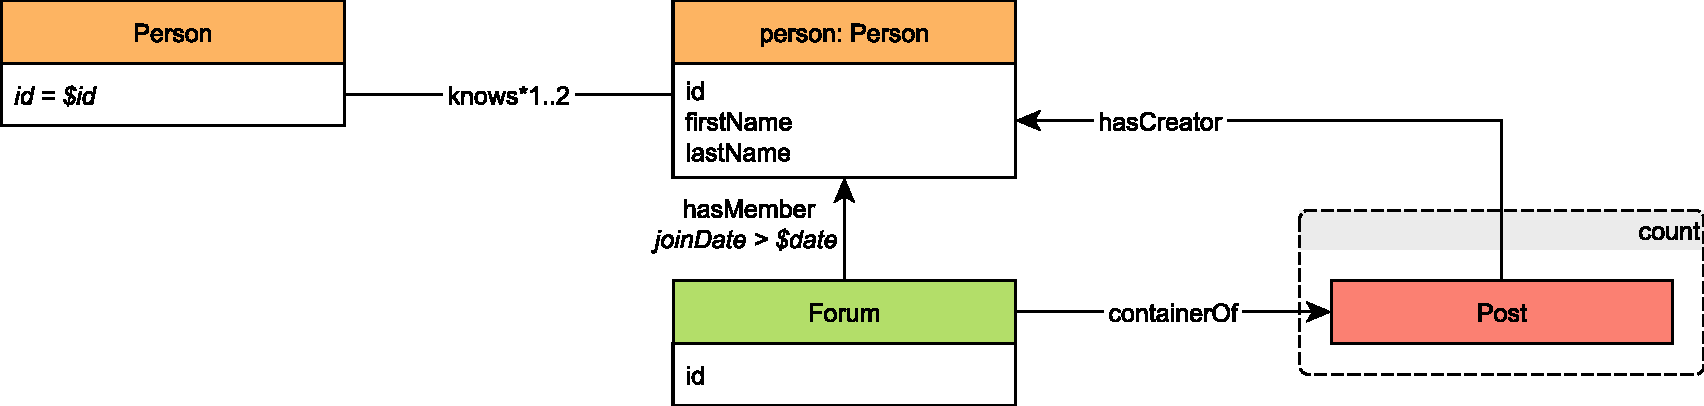
\includegraphics[scale=\patternscale,margin=0cm .2cm]{patterns/interactive-complex-read-05}\hfill\vadjust{} \\ \hline
%
	desc. & Given a start Person, find the Forums which that Person's friends and
friends of friends (excluding start Person) became Members of after a
given date. For each forum find the number of Posts that were created by
any of these Persons. For each Forum and consider only those Persons
which joined that particular Forum after the given date.
 \\ \hline
%
	
		params &
		\innerCardVSpace{\begin{tabularx}{\attributeCardWidth}{|>{\paramNumberCell}c|>{\varNameCell}M|>{\typeCell}m{\typeWidth}|Y|} \hline
		$\mathsf{1}$ & Person.id
 & ID
 &  \\ \hline
		$\mathsf{2}$ & date
 & Date
 &  \\ \hline
		\end{tabularx}}\innerCardVSpace \\ \hline
	
%
	
		result &
		\innerCardVSpace{\begin{tabularx}{\attributeCardWidth}{|>{\resultNumberCell}c|>{\varNameCell}M|>{\typeCell}m{\typeWidth}|>{\resultOriginCell}c|Y|} \hline
		$\mathsf{1}$ & Forum.title & String & R &
				 \\ \hline
		$\mathsf{2}$ & count & 32-bit Integer & A &
				Number of Posts made in Forum that were created by friends
 \\ \hline
		\end{tabularx}}\innerCardVSpace \\ \hline
	
%
	
		sort		&
		\innerCardVSpace{\begin{tabularx}{\attributeCardWidth}{|>{\sortNumberCell}c|>{\varNameCell}M|>{\directionCell}c|Y|} \hline
		$\mathsf{1}$ & count
 & $\desc
$ &  \\ \hline
		$\mathsf{2}$ & Forum.id
 & $\asc
$ &  \\ \hline
		\end{tabularx}}\innerCardVSpace \\ \hline
	%
	limit & 20 \\ \hline
	%
	CPs &
	\multicolumn{1}{>{\raggedright}l|}{
		\chokePoint{2.3}, 
		\chokePoint{3.3}
		} \\ \hline
	%
	relevance &
		\small This query looks for paths of length two and three, starting from a given Person, moving to friends and friends of
friends, and then getting the Forums they are members of. Besides testing the ability of the query optimizer to select
the proper join operator, it rewards the usage of indexes, but their accesses will be presumably scattered due to the
two/three-hop search space of the query, leading to unpredictable and scattered index accesses. Having efficient
implementations of such indexes will be highly beneficial.
 \\ \hline%
\end{tabularx}
\queryCardVSpace

% change \emph back to the old one
\renewcommand{\emph}[1]{\oldemph{#1}}